\section{External stimuli}
\label{sec:external-stimuli}

The external stimulus represents a rectangular grid of non-overlapping equispaced grating annuli - circular Gabor wavelets \cite{MaryamPLACEHOLDER}. The luminance of the stimuli varies between $0$ (black) and $1$ (white), as shown in Figure \ref{fig:full-stimulus-example}. All annuli have equal diameters but vary in contrast. The grid includes a \stimfig{}\footnote{Because of the polysemous nature of the word \say{figure}, it is written in italics when refers to the stimulus \stimfig.} - a rectangular subgrid in the bottom right quadrant of the stimulus, where all annuli share similar contrasts, and a background that constitutes the rest of the grid. There, annuli vary in contrast significantly. The contrast of every annulus is selected at random, depending on the location of the annulus. All areas in the stimulus uncovered by annuli (void) share the same luminance. A square-shaped patch of the stimulus' \stimfig{} is selected as an input to the Izhikevich oscillatory network.

\begin{figure}[!htp]
    \centering
    % ----- INPUT
\newcommand{\fsaimagew}{\textwidth}
\newcommand{\fsaimageh}{\fsaimagew}

% figure center
\newcommand{\fsafigcenterx}{0.68 * \fsaimagew}
\newcommand{\fsafigcentery}{0.2925 * \fsaimageh}

% figure dimensions
\newcommand{\fsafigw}{0.16 * \fsaimagew}
\newcommand{\fsafigh}{0.255 * \fsaimageh}

% patch dimensions
\newcommand{\fsapatchw}{0.1 * \fsaimagew}
\newcommand{\fsapatchh}{0.1 * \fsaimageh}

% shifts
\newcommand{\fsashiftw}{0.03 * \fsaimagew}
\newcommand{\fsashifth}{0.03 * \fsaimageh}

% ----- misc
\newcommand{\fsacenterx}{0.5 * \fsaimagew}
\newcommand{\fsacentery}{0.5 * \fsaimageh}

% figure coords
\newcommand{\fsafigleftx}{\fsafigcenterx - 0.5 * \fsafigw}
\newcommand{\fsafigrightx}{\fsafigcenterx + 0.5 * \fsafigw}
\newcommand{\fsafigtopy}{\fsafigcentery + 0.5 * \fsafigh}
\newcommand{\fsafigbottomy}{\fsafigcentery - 0.5 * \fsafigh}

% patch coords
\newcommand{\fsapatchleftx}{\fsafigcenterx - 0.5 * \fsapatchw}
\newcommand{\fsapatchrightx}{\fsafigcenterx + 0.5 * \fsapatchw}
\newcommand{\fsapatchtopy}{\fsafigcentery + 0.5 * \fsapatchh}
\newcommand{\fsapatchbottomy}{\fsafigcentery - 0.5 * \fsapatchh}

\begin{tikzpicture}[
        arr/.style = { -{Stealth[ ]} },
        whitedoublearrow/.style = {>=stealth, draw=white, fill=white, very thick, <->},
        pinkarrow/.style = {arr, draw=sec-color, fill=sec-color, very thick},
        yellowframe/.style = {rounded corners=0.2cm, very thick, main-color, fill=main-color, fill opacity=0.2},
        blueframe/.style = {rounded corners=0.2cm, very thick, third-color, fill=third-color, fill opacity=0.2},
        anglearrow/.style = {draw, >=stealth, white, very thick, ->, angle eccentricity=2}
    ]
    
    \begin{scope}
        \node[anchor=south west,inner sep=0] at (0,0) {
\includegraphics[width=\fsaimagew]{assets/images/full-stimulus.png}};
        
        % side length
        \node[] (startell) at (0, 0.95 * \fsaimageh) {};
        \node[] (endell) at (\fsaimagew, 0.95 * \fsaimageh) {};
        \path[whitedoublearrow, ultra thick] (startell) edge node {\bgcolorsmalltext{white}{black}{side length $\hat{\ell_\full}, ^\bigcirc$}} (endell);
        
        % center of gaze & stimulsus
        \node[style=cnode] (cent) at (\fsacenterx, \fsacentery) {};
        \node[shift={(-0.5 * \fsacenterx, 0)}] (centtxt) at (\fsacenterx, \fsacentery) {\bgcolorsmalltext{white}{black}{center of gaze \& stimulus $O_{L_\full}$}};
        \path [pinkarrow] (centtxt) edge[bend right=10] node {} (cent);
        
        % figure
        \node[shift={(0, \fsashifth)}] (figuretxt) at (\fsafigcenterx, \fsafigtopy) {\bgcolorsmalltext{white}{black}{figure $F$}};
        \draw[yellowframe] (\fsafigleftx, \fsafigtopy) rectangle (\fsafigrightx, \fsafigbottomy) {};
        
        % figure width
        \node[shift={(0, -1 * \fsashifth)}] (startfigw) at (\fsafigleftx, \fsafigbottomy) {};
        \node[shift={(0, -1 * \fsashifth)}] (endfigw) at (\fsafigrightx, \fsafigbottomy) {};
        
        \path[whitedoublearrow] (startfigw) edge node {\bgcolorsmalltext{white}{black}{$\hat{\ell_{F_w}}, ^\bigcirc$}} (endfigw);
        
        \draw[very thick, white] (\fsafigleftx, \fsafigbottomy) -- (\fsafigleftx, \fsafigbottomy - 2 * \fsashifth);
        \draw[very thick, white] (\fsafigrightx, \fsafigbottomy) -- (\fsafigrightx, \fsafigbottomy - 2 * \fsashifth);
        
        % figure height
        \node[shift={(\fsashiftw, 0)}] (startfigh) at (\fsafigrightx, \fsafigtopy) {};
        \node[shift={(\fsashiftw, 0)}] (endfigh) at (\fsafigrightx, \fsafigbottomy) {};
        
        \path[whitedoublearrow] (startfigh) edge node[rotate=90] {\bgcolorsmalltext{white}{black}{$\hat{\ell_{F_h}}, ^\bigcirc$}} (endfigh);
        
        \draw[very thick, white] (\fsafigrightx, \fsafigtopy) -- (\fsafigrightx + 2 * \fsashiftw, \fsafigtopy);
        \draw[very thick, white] (\fsafigrightx, \fsafigbottomy) -- (\fsafigrightx + 2 * \fsashiftw, \fsafigbottomy);
        
        % patch
        \node[shift={(0, \fsashifth)}] (patchtxt) at (\fsafigcenterx, \fsapatchtopy) {\bgcolorsmalltext{white}{black}{patch $L$}};
        \draw[blueframe] (\fsapatchleftx, \fsapatchtopy) rectangle (\fsapatchrightx, \fsapatchbottomy) {};
        
        % center of figure & patch
        \node[shift={(-0.3 * \fsaimagew, -0.1 * \fsaimageh)}] (cent2txt) at (\fsafigcenterx, \fsafigcentery) {\bgcolorsmalltext{white}{black}{center of figure \& patch $F_O$}};
        \node[style=cnode] (cent2) at (\fsafigcenterx, \fsafigcentery) {};
        \path [pinkarrow] (cent2txt) edge[bend right=10] node {} (cent2);
        
        % eccentricity
        \path[whitedoublearrow] (cent) edge node[sloped] {\bgcolorsmalltext{white}{black}{$\hat{\ecc_F}, ^\bigcirc$}} (cent2);
        
        % angle
        \draw[main-color] (\fsacenterx, \fsacentery) -- (\fsaimagew, \fsacentery);
        \node[] (xright) at (\fsaimagew, \fsacentery) {};
        \pic[anglearrow, "\bgcolorsmalltext{white}{black}{$\; \theta \;$}"] {angle = cent2--cent--xright};
        
        
    \end{scope}
\end{tikzpicture}
    \caption[Full stimulus annotated]{An example of the full stimulus with parameters $ \spatfreq = 5.7 \text{ cycles}/\circ, \vlum = 0.5, \diamdg = 0.7^\circ, \diam = 48, \anndistscale = 1, \fullwidthdg = 33.87^\circ, \fullheightdg = 27.09^\circ, \contrange = 0.01, \figwidthdg = 5^\circ, \figheightdg = 9^\circ, \figeccdg = 11^\circ, \patchsizedg = 4.9^\circ$.}
    \label{fig:full-stimulus-example}
\end{figure}

\subsection{Luminance stimulus construction}
\label{sec:luminance-stim-construction}

The composition of the stimulus is a rather involved process, which can be separated in the following simpler steps:
\begin{enumerate}
    \item construction of the Gabor annulus with maximal contrast; \\
    First, the distance from the annulus center at every pixel is computed. The pixels where this distance is smaller than the given radius of the annulus are assigned the Gabor grating luminance; others are assigned the designated void value. For more details, see Section \ref{sec:annulus-composition}.
    
    \item determining the position and coordinates of the \stimfig{} in the stimulus; \\
    We start by selecting a random position of the \stimfig{} within the stimulus given the \stimfig{} size and its distance from the center of the stimulus. From there, the center of the \stimfig{} and its pixel coordinates are computed. For more details, see Section \ref{sec:figure-composition}.
    
    \item positioning of the copies of the Gabor annulus in the stimulus; \\
    At this step, we first determine the distance between the neighboring annuli in the grid, which is equal to the number of pixels allocated to each annulus and void around it. Then, the number of annuli in each grid row and column is determined. Finally, the set of all annuli's left top corners (starting points) is computed. For more details, see Section \ref{sec:annuli-locations}.
    
    \item assigning random contrasts to the different stimulus areas (\stimfig, ground, void) depending on their location; \\
    First, the stimulus is initialized with the void luminance. Then, the annuli with relevant contrasts are added to the matrix at locations determined in the previous step. If an annulus is located in the
    ground, its contrast is selected randomly from the range $[0, 1]$, otherwise, if it is located in the \stimfig, the contrast is selected from a smaller range. For more details, see Section \ref{sec:luminance-assignment}.
    
    \item selecting a patch from the figure for further processing. \\
    Given the patch dimensions, its concentricness to the \stimfig, and lower right quadrant location, we determine the luminance matrix of the patch.
    For more details, see Section \ref{sec:patch-selection}.
\end{enumerate}

The result of completing the aforementioned steps includes a stimulus luminance matrix and a \stimfig{} patch, examples of which are displayed in Figure \ref{fig:full-stimulus-example} and Figure \ref{fig:stim-patch-example}, respectively.

\subsubsection{Input parameters}
\label{sec:stimulus-parameters}

The appearance of the stimulus depends on many input parameters.
The reader may omit this section as the parameters are explained as they appear in the text. The summary list below is presented for convenience.

All spatial parameters are given in visual degrees: $1^\circ$ is equivalent to $1$ cm when the distance between the visual field and an eye is $37.5$ cm. For one such parameter (annulus diameter), the input is provided in pixels, too, allowing for scaling other parameters. The values given in visual degrees are further referred to as physical, and the pixel values - naturally, as pixel.

For the construction of an annulus, the following parameters are given:
\begin{itemize}
    \item $\spatfreq \in \mathbb{R}_+$ - the spatial frequency in cycles per degree;
    
    \item $\vlum \in [0, 1]$ - the void luminance value;
    
    \item $\diamdg \in \mathbb{R}_+$ - the diameter of a single annulus in visual degrees;
    
    \item $\diam \in \mathbb{N}$ - the diameter of a single annulus in pixels.
\end{itemize}
Since the mapping of the physical space (degrees) to pixel values in isomorphic, a conversion coefficient $\atopix \in \mathbb{R}_+$ between the two can be defined as follows:
\begin{equation}
    \atopix = \frac{\diam}{\diamdg}.
\end{equation}

The parameters relevant for the full stimulus are
\begin{itemize}
    \item $\anndistscale \in [1, \infty)$ - the scalar that represents the distance scale between neighboring annuli (the minimum possible value is $1$ to ensure the annuli do not overlap);
    
    \item $\fullwidthdg \in [\diam, \infty)$ - the width of the stimulus in visual degrees; in pixels, the width is
    $
        \fullwidth = \ceil{\atopix \cdot \fullwidthdg};
    $
    
    \item $\fullheightdg \in [\diam, \infty)$ - the height of the stimulus in visual degrees; in pixels, the height is
    $
        \fullheight = \ceil{\atopix \cdot \fullheightdg}.
    $
\end{itemize}

The parameters relevant for the figure are
\begin{itemize}

    \item $\contrange \in (0, 1]$ - the range of annuli contrasts in the figure;
    
    \item $\figwidthdg \in (0, \frac{1}{2} \fullwidthdg]$ - the width of the figure in visual degrees (must fit in the bottom right quadrant of the stimulus); in pixels, the width is
    $
        \figwidth = \ceil{\atopix \cdot \figwidthdg};
    $
    
    \item $\figheightdg \in (0, \frac{1}{2} \fullheightdg]$ - the height of the figure in visual degrees; in pixels, the width is
    $
        \figheight = \ceil{\atopix \cdot \figheightdg};
    $
    
    \item $\figeccdg \in [\figdiag, \| (\frac{1}{2} \fullwidthdg, \frac{1}{2} \fullheightdg)\| - \figdiag]$, where
    \begin{equation}
        \figdiag = \left\| 
            \left(
                \frac{1}{2} \figwidthdg, 
                \frac{1}{2} \figheightdg 
            \right)
        \right\|,
        \label{eq:figdiag}
    \end{equation}
    - the distance between the center of the stimulus and the center of the figure in visual degrees; in pixels, this distance is
    $
        \figecc = \ceil{\atopix \cdot \figeccdg}.
    $
\end{itemize}

Finally, the parameter for the stimulus patch is
\begin{itemize}

    \item $n \in \mathbb{N}$ - the number of PING networks in each dimension of the oscillatory network, as shown in Section \ref{sec:grid-network};
    
    \item $\patchsizedg \in (0, \min(\figwidthdg, \figheightdg)]$ - the side length of the stimulus patch in visual degrees; in pixels, the length is
    $
        \patchsize = \ceil{\atopix \cdot \patchsizedg}.
    $
    Additionally, for further processing, $(n | \patchsize)$ must hold.
\end{itemize}

The parameters' values used for composing the stimuli are displayed in Table \ref{tab:stimulus-composition-params}.

\begin{table}[!htp]
    \centering
    \begin{tabular}{|
>{\columncolor{main-color}}c |ccccc|}
\hline
\textbf{Parameter}      & \multicolumn{5}{c|}{\cellcolor{main-color}\textbf{Value(s)}}                                                                      \\ \hline
\textbf{$\pmb{\hat{d}}$}      & \multicolumn{5}{c|}{$0.7^\circ$}                                                                                                    \\ \hline
$\pmb{\vlum}$           & \multicolumn{5}{c|}{$0.5$}                                                                                                          \\ \hline
\textbf{$\pmb{\Omega}$} & \multicolumn{5}{c|}{$5.7$ cycles/degree}                                                                                            \\ \hline
$\pmb{\hat{\ell_{F_w}}}$      & \multicolumn{5}{c|}{$(9 \pm 0.7)^\circ$}                                                                                            \\ \hline
$\pmb{\hat{\ell_{F_h}}}$      & \multicolumn{5}{c|}{$(5 \pm 0.4)^\circ$}                                                                                            \\ \hline
$\pmb{\hat{\ecc_F}}$          & \multicolumn{5}{c|}{$(7 \pm 1)^\circ$}                                                                                              \\ \hline
$\pmb{k}$               & \multicolumn{1}{c|}{$1$}    & \multicolumn{1}{c|}{$1.125$}  & \multicolumn{1}{c|}{$1.250$}  & \multicolumn{1}{c|}{$1.375$}  & $1.5$ \\ \hline
$\pmb{\eta}$            & \multicolumn{1}{c|}{$0.01$} & \multicolumn{1}{c|}{$0.0257$} & \multicolumn{1}{c|}{$0.5050$} & \multicolumn{1}{c|}{$0.7525$} & $1$   \\ \hline
\end{tabular}
    \caption[Stimuli parameters]{The values of the parameters used to generate texture stimuli. The parameters are chosen to be either identical or close to \cite{MaryamPLACEHOLDER}.}
    \label{tab:stimulus-composition-params}
\end{table}
\subsubsection{Annulus composition}
\label{sec:annulus-composition}

Let $\annradii \in [0, 1]^{\diam \times \diam}$ be a matrix containing the distances (radii) of each pixel from the middle of the matrix. If $\diam = 1$,
\begin{equation}
    \annradii = 
    \begin{pmatrix}
        0
    \end{pmatrix}.
\end{equation}
Otherwise, for $i, j \in \{ 0, 1, \cdots,  \diam-1 \}$,
\begin{equation}
    \annradii_{i, j} = \left\| 
        (0, 0), \ 
        \left(
            -\frac{\diamdg}{2} + \frac{\diamdg}{\diam - 1} i, 
            -\frac{\diamdg}{2} + \frac{\diamdg}{\diam - 1} j 
        \right) 
    \right\|.
\end{equation}

Let $\annmatrix \in [0, 1]^{\diam \times \diam}$ be the pixel luminance matrix of the annulus. Then, for $i, j \in \{ 0, 1, \cdots,  \diam-1 \}$,
\begin{equation}
    \annmatrix_{i, j} = \vlum \cdot
    \begin{cases}
        \cos(2 \pi \annradii_{i, j} \spatfreq + \pi) 
        &\text{ if } \annradii_{i, j} \leq \frac{\diamdg}{2} \\
        1 
        &\text{ otherwise}
    \end{cases},
    \label{eq:grating}
\end{equation}
where $\vlum \in [0, 1]$ is luminance of the void (the area uncovered by the annulus).
An example of the resulting luminance matrix' binary heat map is visualized in Figure \ref{fig:grating-example}.

\begin{figure}[!htp]
    \centering
    
\includegraphics[width=0.2\textwidth]{assets/images/grating.png}
    \caption{An example of the annulus grating with maximal contrast and $\spatfreq = 5.7 \text{ cycles}/\circ, \vlum = 0.5, \diamdg = 0.7^\circ, \diam = 50$.}
    \label{fig:grating-example}
\end{figure}
\subsubsection{Figure composition}
\label{sec:figure-composition}

Let $\fullmatrix \in [0, 1]^{\fullwidth \times \fullheight}$ be the matrix allocated for the stimulus' luminance values, where $\fullwidth, \fullheight \in [\diam, \infty)$ represent the stimulus width and height, respectively.
Let $\figwidth \in (0, \frac{1}{2} \fullwidthdg]$ be the \stimfig{} width, and $\figheight \in (0, \frac{1}{2} \fullheightdg]$ - its height. The \stimfig{} comprises a submatrix of the full stimulus $\fullmatrix$. The \stimfig{} is located at the pixel distance $\figecc$ from the stimulus center, as defined in Equation (\ref{eq:figdiag}), at an angle $\figangle \sim U(\figanglemin, \figanglemax)$ to the horizontal axis. Since the \stimfig{} is located in the bottom right quadrant,
\begin{equation}
    \begin{aligned}
        \figanglemin &=
        \begin{cases}
            \cos^{-1} \left(
                \frac{\fullwidth - \figwidth}{2 \cdot \figecc}
            \right)
            &\text{ if } \figecc > \frac{\fullwidth - \figwidth}{2} \\
            \sin^{-1} \left( 
                \frac{\figheight}{2 \cdot \figecc}
            \right)
            &\text{ otherwise}
        \end{cases}, \\
        \figanglemax &= \frac{\pi}{2} - 
        \begin{cases}
            \cos^{-1} \left(
                \frac{\fullheight - \figheight}{2 \cdot \figecc}
            \right)
            &\text{ if } \figecc > \frac{\fullheight - \figheight}{2} \\
            \sin^{-1} \left( 
                \frac{\figwidth}{2 \cdot \figecc}
            \right)
            &\text{ otherwise}
        \end{cases}.
    \end{aligned}
\end{equation}
Now, we can locate the center of the \stimfig{} $\figcenter \in \mathbb{R}_+^2$:
\begin{equation}
    \figcenter = \left(
        \frac{1}{2} \fullwidth + \figecc \cdot \cos(\figangle), \
        \frac{1}{2} \fullheight + \figecc \cdot \sin(\figangle)
    \right).
\end{equation}
The center of the \stimfig{} need not be integer as it is only used for determining the \stimfig{}'s top left ($\figstart \in \mathbb{N}^2$) and bottom right ($\figfinish \in \mathbb{N}^2$) coordinates:
\begin{align}
\begin{split}
    \figstart &= \ceil{\figcenter - \frac{1}{2} (\figheight, \figwidth)}, \\
    \figfinish &= \figstart + (\figheight, \figwidth),
\end{split}
\label{eq:figure-location}
\end{align}
The ceiling function in Equation (\ref{eq:figure-location}) is applied element-wise.
\subsubsection{Annuli locations}
\label{sec:annuli-locations}

The distance between the centers of neighboring annuli is
\begin{equation}
    \anndist = \ceil{\anndistscale \cdot \diam}.
\end{equation}
The variable $\anndist \in \mathbb{N}$ then also indicates the number of pixels allocated to each annulus and void around it. Consequently, we can determine the number of annuli that are (partially) located in each row $\repsinrow \in \mathbb{N}$ and column $\repsincol \in \mathbb{N}$ of the stimulus:
\begin{equation}
    \repsinrow = \ceil{\frac{\fullwidth}{\anndist}}, \;
    \repsincol = \ceil{\frac{\fullheight}{\anndist}}. 
\end{equation}

Let $\annuliset$ be the set containing all matrices associated with annuli in $\fullmatrix$. Then, $|\annuliset| = \repsinrow \cdot \repsincol$, and
\begin{equation}
\begin{gathered}
    \annuliset \coloneqq \bigcup_{i = 0}^{\repsinrow - 1} \bigcup_{j = 0}^{\repsincol - 1}
    \begin{pmatrix}
        \fullmatrix_{\annstart_{\annuliset_{i, j}}} & & \\
         & \ddots & \\
         & & \fullmatrix_{\annfinish_{\annuliset_{i, j}}}
    \end{pmatrix}, \\
    \begin{aligned}
    \annstart_{\annuliset_{i, j}} &= \left( 
        i \cdot \anndist + \floor{ \frac{1}{2} (\anndist - \diam) }, \ 
        j \cdot \anndist + \floor{ \frac{1}{2} (\anndist - \diam) }
    \right), \\
    \annfinish_{\annuliset_{i, j}} &=
    \min(
        \annstart_{\annuliset_{i, j}} + (d, d), \ 
        (\fullwidth, \fullheight)
    ),
    \end{aligned}
\end{gathered}
\end{equation}
where $\annstart_{\annuliset_{i, j}}, \annfinish_{\annuliset_{i, j}} \in \mathbb{N}^2$ are the top left and bottom right coordinates of an annulus $\annuliset_{i, j} \in \annuliset$, respectively. 

As we position the annuli in the middle of the allocated space, for each stimulus, there exist values of $\anndistscale$, such that the last annulus in a row or column starts outside of the bounds of the figure. Such annuli need to be removed from the set $\annuliset$:
\begin{equation}
    \annuliset \leftarrow \annuliset \setminus \{ \annstimmatrix \in \annuliset \ | \ \annstart_\annstimmatrix > (\fullwidth, \fullheight) \}
\end{equation}
\subsubsection{Luminance assignment}
\label{sec:luminance-assignment}

First, all values of the stimulus $\fullmatrix$ are initialized with the void luminance $\vlum$. Then, the annuli with relevant contrasts are added to the matrix. Let $\view: \annuliset \to \{ \fig, \ground \}$ be the function mapping an annulus to its view. Let $\annstimmatrix \in \annuliset$, then
\begin{equation}
    \view(\annstimmatrix) = 
    \begin{cases}
        \fig & \text{ if } 
        \{ \annstart_\annstimmatrix, \cdots,  \annfinish_\annstimmatrix \}
        \cap
        \{ \figstart, \cdots, \figfinish \}
        \neq \emptyset \\
        \ground & \text{ otherwise} 
    \end{cases}.
\end{equation}
So, an annulus is said to be located in the figure if it is (partially) contained in it.

Let $\unirand: \annuliset \to U(0, 1)$ be a random value that varies per annulus. The values are independent and identically distributed (i.i.d.). Then for all $\annstimmatrix \in \annuliset$ and $\lambda, \mu \in \{ 0, 1, \cdots, \diam - 1\}, \ (i, j) = \annstart_\annstimmatrix + (\lambda, \mu)$,
\begin{equation}
    \fullmatrix_{i, j} \leftarrow \vlum +
    \begin{cases}
        (\annmatrix_{\lambda, \mu} - \vlum) \cdot \left( \unirand(\annstimmatrix) \contrange + \vlum \cdot (1 - \contrange) \right) 
        &\text{ if } \view(\annstimmatrix) = \fig  \\
        (\annmatrix_{\lambda, \mu} - \vlum) \cdot \unirand(\annstimmatrix) 
        &\text{ otherwise}
    \end{cases}.
\end{equation}
Now, the stimulus luminance matrix is complete.
Thus, the luminance of the void, similar to annuli's edges as demonstrated in Equation (\ref{eq:grating}), are still assigned the luminance of $\vlum$; the mean of all pixels' luminance values is also equal to $\vlum$. An example of the resulting luminance matrix' binary heat map is visualized in Figure \ref{fig:full-stimulus-example}.

\begin{figure}[!htp]
    \centering
    % ----- INPUT
\newcommand{\fsaimagew}{\textwidth}
\newcommand{\fsaimageh}{\fsaimagew}

% figure center
\newcommand{\fsafigcenterx}{0.68 * \fsaimagew}
\newcommand{\fsafigcentery}{0.2925 * \fsaimageh}

% figure dimensions
\newcommand{\fsafigw}{0.16 * \fsaimagew}
\newcommand{\fsafigh}{0.255 * \fsaimageh}

% patch dimensions
\newcommand{\fsapatchw}{0.1 * \fsaimagew}
\newcommand{\fsapatchh}{0.1 * \fsaimageh}

% shifts
\newcommand{\fsashiftw}{0.03 * \fsaimagew}
\newcommand{\fsashifth}{0.03 * \fsaimageh}

% ----- misc
\newcommand{\fsacenterx}{0.5 * \fsaimagew}
\newcommand{\fsacentery}{0.5 * \fsaimageh}

% figure coords
\newcommand{\fsafigleftx}{\fsafigcenterx - 0.5 * \fsafigw}
\newcommand{\fsafigrightx}{\fsafigcenterx + 0.5 * \fsafigw}
\newcommand{\fsafigtopy}{\fsafigcentery + 0.5 * \fsafigh}
\newcommand{\fsafigbottomy}{\fsafigcentery - 0.5 * \fsafigh}

% patch coords
\newcommand{\fsapatchleftx}{\fsafigcenterx - 0.5 * \fsapatchw}
\newcommand{\fsapatchrightx}{\fsafigcenterx + 0.5 * \fsapatchw}
\newcommand{\fsapatchtopy}{\fsafigcentery + 0.5 * \fsapatchh}
\newcommand{\fsapatchbottomy}{\fsafigcentery - 0.5 * \fsapatchh}

\begin{tikzpicture}[
        arr/.style = { -{Stealth[ ]} },
        whitedoublearrow/.style = {>=stealth, draw=white, fill=white, very thick, <->},
        pinkarrow/.style = {arr, draw=sec-color, fill=sec-color, very thick},
        yellowframe/.style = {rounded corners=0.2cm, very thick, main-color, fill=main-color, fill opacity=0.2},
        blueframe/.style = {rounded corners=0.2cm, very thick, third-color, fill=third-color, fill opacity=0.2},
        anglearrow/.style = {draw, >=stealth, white, very thick, ->, angle eccentricity=2}
    ]
    
    \begin{scope}
        \node[anchor=south west,inner sep=0] at (0,0) {
\includegraphics[width=\fsaimagew]{assets/images/full-stimulus.png}};
        
        % side length
        \node[] (startell) at (0, 0.95 * \fsaimageh) {};
        \node[] (endell) at (\fsaimagew, 0.95 * \fsaimageh) {};
        \path[whitedoublearrow, ultra thick] (startell) edge node {\bgcolorsmalltext{white}{black}{side length $\hat{\ell_\full}, ^\bigcirc$}} (endell);
        
        % center of gaze & stimulsus
        \node[style=cnode] (cent) at (\fsacenterx, \fsacentery) {};
        \node[shift={(-0.5 * \fsacenterx, 0)}] (centtxt) at (\fsacenterx, \fsacentery) {\bgcolorsmalltext{white}{black}{center of gaze \& stimulus $O_{L_\full}$}};
        \path [pinkarrow] (centtxt) edge[bend right=10] node {} (cent);
        
        % figure
        \node[shift={(0, \fsashifth)}] (figuretxt) at (\fsafigcenterx, \fsafigtopy) {\bgcolorsmalltext{white}{black}{figure $F$}};
        \draw[yellowframe] (\fsafigleftx, \fsafigtopy) rectangle (\fsafigrightx, \fsafigbottomy) {};
        
        % figure width
        \node[shift={(0, -1 * \fsashifth)}] (startfigw) at (\fsafigleftx, \fsafigbottomy) {};
        \node[shift={(0, -1 * \fsashifth)}] (endfigw) at (\fsafigrightx, \fsafigbottomy) {};
        
        \path[whitedoublearrow] (startfigw) edge node {\bgcolorsmalltext{white}{black}{$\hat{\ell_{F_w}}, ^\bigcirc$}} (endfigw);
        
        \draw[very thick, white] (\fsafigleftx, \fsafigbottomy) -- (\fsafigleftx, \fsafigbottomy - 2 * \fsashifth);
        \draw[very thick, white] (\fsafigrightx, \fsafigbottomy) -- (\fsafigrightx, \fsafigbottomy - 2 * \fsashifth);
        
        % figure height
        \node[shift={(\fsashiftw, 0)}] (startfigh) at (\fsafigrightx, \fsafigtopy) {};
        \node[shift={(\fsashiftw, 0)}] (endfigh) at (\fsafigrightx, \fsafigbottomy) {};
        
        \path[whitedoublearrow] (startfigh) edge node[rotate=90] {\bgcolorsmalltext{white}{black}{$\hat{\ell_{F_h}}, ^\bigcirc$}} (endfigh);
        
        \draw[very thick, white] (\fsafigrightx, \fsafigtopy) -- (\fsafigrightx + 2 * \fsashiftw, \fsafigtopy);
        \draw[very thick, white] (\fsafigrightx, \fsafigbottomy) -- (\fsafigrightx + 2 * \fsashiftw, \fsafigbottomy);
        
        % patch
        \node[shift={(0, \fsashifth)}] (patchtxt) at (\fsafigcenterx, \fsapatchtopy) {\bgcolorsmalltext{white}{black}{patch $L$}};
        \draw[blueframe] (\fsapatchleftx, \fsapatchtopy) rectangle (\fsapatchrightx, \fsapatchbottomy) {};
        
        % center of figure & patch
        \node[shift={(-0.3 * \fsaimagew, -0.1 * \fsaimageh)}] (cent2txt) at (\fsafigcenterx, \fsafigcentery) {\bgcolorsmalltext{white}{black}{center of figure \& patch $F_O$}};
        \node[style=cnode] (cent2) at (\fsafigcenterx, \fsafigcentery) {};
        \path [pinkarrow] (cent2txt) edge[bend right=10] node {} (cent2);
        
        % eccentricity
        \path[whitedoublearrow] (cent) edge node[sloped] {\bgcolorsmalltext{white}{black}{$\hat{\ecc_F}, ^\bigcirc$}} (cent2);
        
        % angle
        \draw[main-color] (\fsacenterx, \fsacentery) -- (\fsaimagew, \fsacentery);
        \node[] (xright) at (\fsaimagew, \fsacentery) {};
        \pic[anglearrow, "\bgcolorsmalltext{white}{black}{$\; \theta \;$}"] {angle = cent2--cent--xright};
        
        
    \end{scope}
\end{tikzpicture}
    \caption{An example of the full stimulus with parameters $ \spatfreq = 5.7 \text{ cycles}/\circ, \vlum = 0.5, \diamdg = 0.7^\circ, \diam = 48, \anndistscale = 1, \fullwidthdg = 33.87^\circ, \fullheightdg = 27.09^\circ, \contrange = 0.01, \figwidthdg = 5^\circ, \figheightdg = 9^\circ, \figeccdg = 11^\circ, \patchsizedg = 4.9^\circ$.}
    \label{fig:full-stimulus-example}
\end{figure}
\subsubsection{Patch selection}
\label{sec:patch-selection}

A square patch $\patchmatrix \in [0, 1]^{\patchsize \times \patchsize}$ is concentric to the figure $\figmatrix$. Thus, it can be defined as
\begin{equation}
    \patchmatrix \coloneqq 
    \begin{pmatrix}
        \fullmatrix_{\ceil{ \figcenter - \frac{\patchsize}{2}}, \ceil{  \figcenter - \frac{\patchsize}{2} }} &  &  \\
         & \ddots &  \\
         &  &  \fullmatrix_{\ceil{ \figcenter - \frac{\patchsize}{2}} + \ell, \ceil{  \figcenter - \frac{\patchsize}{2}} + \ell}
    \end{pmatrix}.
\end{equation}
An example of the resulting binary heat map of the texture stimulus patch is visualized in Figure \ref{fig:stim-patch-example}.

\begin{figure}
    \centering
    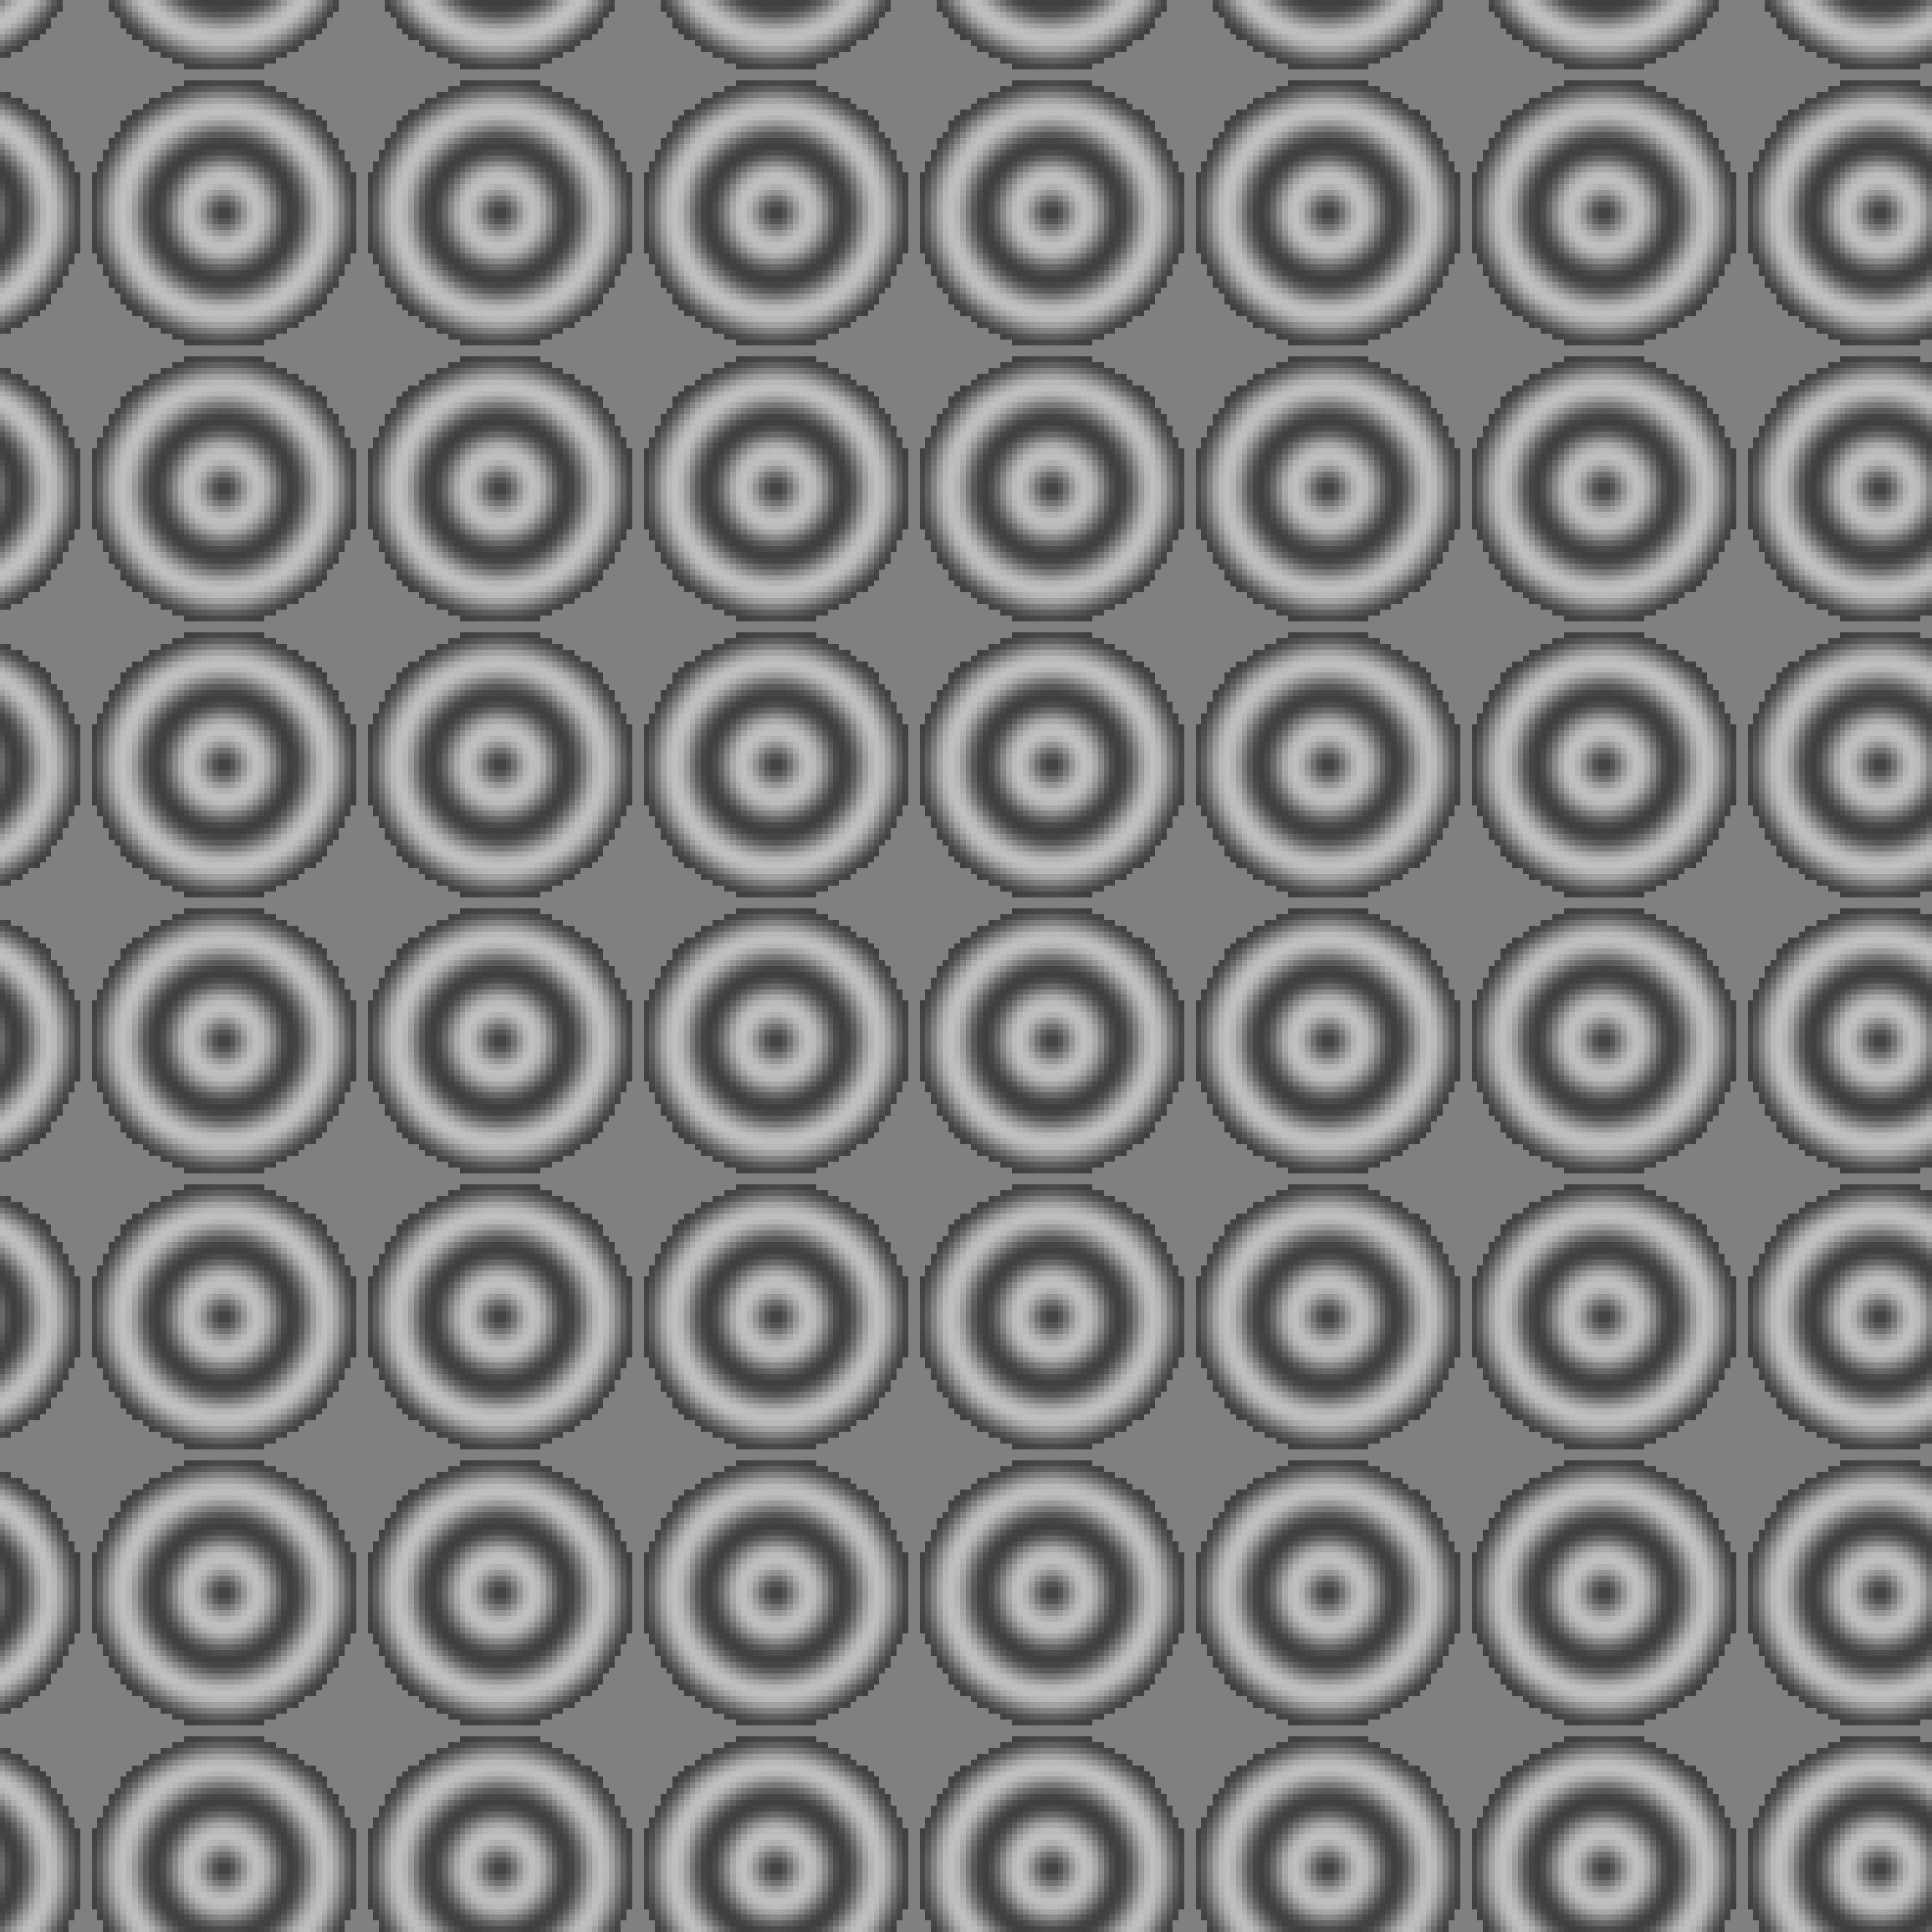
\includegraphics[width=0.4\textwidth]{src/assets/images/stimulus-patch.png}
    \caption{The stimulus patch obtained from Figure \ref{fig:full-stimulus-example}.}
    \label{fig:stim-patch-example}
\end{figure}







\subsection{Set of stimuli}

\todo{write this}


\subsection{Current from stimulus}

\subsubsection{From luminance to contrast}

To transform the stimulus patch $\patchmatrix$ to the patch of PING networks in V1, we apply the lattice of size $n \times n$, such that each oscillatory network contains a field of $m \times m$ pixels. An example of the resulting lattice is displayed in Figure \ref{fig:llc-lattice-example}.


\begin{figure}[!htp]
    \centering
    \begin{subfigure}[t]{0.4\textwidth}
        \centering
        \newcommand{\splw}{\textwidth}
\newcommand{\splh}{\splw}

\newcommand{\splnrverticallines}{11}
\newcommand{\splverticalinterval}{0.08333} % 1 / (splnrverticallines + 1)

\newcommand{\splnrhorizontallines}{11}
\newcommand{\splhorizontalinterval}{0.08333}

\begin{tikzpicture}[
    cline/.style = {very thick, color-one},
]
    \begin{scope}
        \node[anchor=south west,inner sep=0] at (0,0) {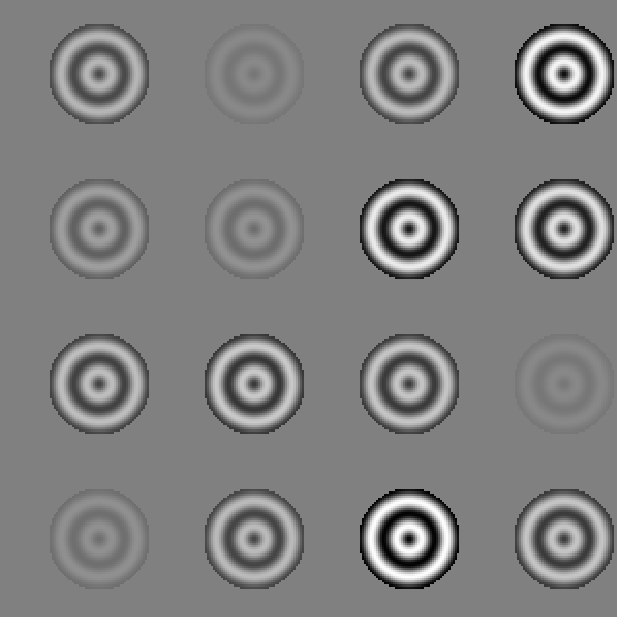
\includegraphics[width=\splw]{src/assets/images/stimulus-patch-lattice.png}};
        
        % vertical
        \foreach \i in {1, 2, ..., \splnrverticallines}{
            \draw[cline] (\i * \splverticalinterval * \splw, 0) -- (\i * \splverticalinterval * \splw, \splh) {};
        }
        
        % horizontal
        \foreach \i in {1, 2, ..., \splnrverticallines}{
            \draw[cline] (0, \i * \splhorizontalinterval * \splh) -- (\splw, \i * \splhorizontalinterval * \splh) {};
        }

    \end{scope}
\end{tikzpicture}
        \caption{A 20 $\times$ 20 lattice applied to a patch.}
        \label{fig:llc-lattice-example}
    \end{subfigure}
    \hspace{0.06\textwidth}
    \begin{subfigure}[t]{0.4\textwidth}
        \centering
        
\includegraphics[width=\textwidth]{src/assets/images/local-contrast.png}
        \caption{Local contrasts of the patch in Figure \ref{fig:llc-lattice-example}: $0$ (black) $\to$ $1$ (white).}
        \label{fig:llc-local-contrast-example}
    \end{subfigure}
    \caption[Patch lattice and local contrast]{The lattice of a patch and its vertices' local contrasts. 
    The patch was generated with the parameters $\anndistscale = 1.5$, $\contrange = 1$.}
    \label{fig:lattice-local-contrast-example}
\end{figure}


Let $\pingnets$ be the set containing the PING networks. Let $\pix: \pingnets \to (\mathbb{Z}_+)^{2 \times m^2}$ be a function mapping a network to the set of all $m^2$ pixel coordinates it contains.
For each network $\pingnet \in \pingnets$, a local contrast $\LC: V \to \mathbb{R}$ is the weighted root-mean-squared (RMS) contrast defined as follows \cite{Frazor2006}:
\begin{equation}
    \LC_\pingnet = \sqrt{
        \frac{
            \sum_{(i, j) \in \patchmatrix} \weight_{\pingnet, (i, j)} \frac{(\patchmatrix_{i, j} - \overline{\fullmatrix})^2}{\overline{\fullmatrix}^2}
        }{
            \sum_{(i, j) \in \patchmatrix} \weight_{\pingnet, (i, j)}
        }
    },
\end{equation}
\begin{comment}
\begin{equation}
    \LC_\pingnet = \sqrt{
        \frac{
            \sum_{(i, j) \in \pix(\pingnet)} \weight_{\pingnet, (i, j)} \frac{(\patchmatrix_{i, j} - \overline{\fullmatrix})^2}{\overline{\fullmatrix}^2}
        }{
            \sum_{(i, j) \in \pix(\pingnet)} \weight_{\pingnet, (i, j)}
        }
    },
\end{equation}
\end{comment}
where $\overline{\fullmatrix}$ is the mean over all luminance values in $\fullmatrix$, and $\weight: \pingnets, \mathbb{N}^2 \to \mathbb{R}$ is the weight of a pixel with respect to a network, as shown in Equation (\ref{eq:weight-pixel-network}). An example of a local contrast matrix can be seen in Figure \ref{fig:llc-local-contrast-example}.

To define that weight, one first needs to complete a number of steps.
Let $\centr : \pingnets \to \mathbb{R}_+^2$ be the function mapping a particular PING network in the patch to the location of its center. As the center of the gaze (fovea) coincides with the center of the stimulus, the eccentricity $\ecc: \pingnets \to \mathbb{R}_+$ in degrees for a network $v \in \pingnets$ is
\begin{equation}
\begin{gathered}
    \ecc_{\pingnet} = \frac{1}{\atopix} \cdot \left\| \stimcenter, \ \patchstart + \centr(\pingnet) \right\|, \\
    \stimcenter = \left( \frac{\fullwidth}{2}, \frac{\fullheight}{2}   \right).
\end{gathered}
\end{equation}

Let $\slopeRF \in \mathbb{R}$ be the slope, the ratio of receptive field diameter to eccentricity, and $\interceptRF \in \mathbb{R}$ - the intercept \cite{Freeman2011, MaryamPLACEHOLDER}.
Let $\diamRF_{\min} \in \mathbb{R}_+$ be smallest allowed diameter of the receptive field.
Then, the diameter of the receptive field $\diamRF \in \mathbb{R}$ of $\pingnet$ is 
\begin{equation}
    \diamRF_\pingnet = \max{( \slopeRF \cdot \ecc_\pingnet + \interceptRF, \ \diamRF_{\min} )}.
\end{equation}

Let $\stdrf: \pingnets \to \mathbb{R}$ be the standard deviation of the receptive field diameter of a Gaussian beam \cite{MaryamPLACEHOLDER}. It can be obtained by utilizing the full width at half maximum $\fwhm: \pingnets \to \mathbb{R}$ in the following way:
\begin{equation}
    \begin{cases}
        \fwhm_\pingnet = \sqrt{\frac{\ln(2)}{2}} \cdot \diamRF_\pingnet \\
        \fwhm_\pingnet = 2 \sqrt{2 \ln(2)} \cdot \stdrf_\pingnet
    \end{cases}
    \Rightarrow 
    \stdrf_\pingnet = \frac{1}{4} \diamRF_\pingnet.
\end{equation}

Having derived the standard deviation, the weight of the pixel $i, j \in \{ 0, 1, \cdots, \patchsize - 1 \}$ with respect to a PING network $\pingnet$ can be defined at last. This value is specific to each network as it reflects its unique receptive field modeled with an isotropic 2D Gaussian function \cite{MaryamPLACEHOLDER}:
\begin{equation}
    \weight_{\pingnet, (i, j)} = \exp \left(
        -\frac{\left( \frac{1}{\atopix} \cdot \| (i, j), \ \centr(\pingnet) \|\right)^2}{ 2 \stdrf_\pingnet^2 }
    \right).
    \label{eq:weight-pixel-network}
\end{equation}
\subsubsection{From contrast to frequency}

Now, the oscillation frequency $f$ of the PING network $\pingnet$ can be obtained through the local contrast:
\begin{equation}
    f_\pingnet = 25 + 0.25 \cdot \LC_\pingnet.
\end{equation}
These relations reflect the typical gamma frequency of a neural network in V1.
\subsubsection{From frequency to current}

This section describes a method for determining the relationship between gamma frequencies and input currents. It involves simulating the network using the Izhikevich model with different currents and constructing a time-frequency representation (TFR) of the resulting spike trains using the Morlet wavelet transform. The dominant frequency of gamma oscillations in the signal can be determined from the TFR. The dominant frequency for each simulation is then plotted against the corresponding input current to find the relationship between current and frequency.

\paragraph{Simulating with different currents}

To collect the required data for a given input current, we simulate the Izhikevich model with the previously introduced parameters (see Section \ref{sec:grid-network}). Instead of the current input from an external stimulus, $I_\stim$ in Equation (\ref{eq:current-components}), current $I_\inpt$ is used:
\begin{equation}
    I_{\inpt, v} = \begin{cases}
        \meancurrent_\ex & \text{ if } \type(v) = \ex \\
        \meancurrent_\inh & \text{ if } \type(v) = \inh
    \end{cases}.
\end{equation}
The input current to inhibitory neurons $\meancurrent_\inh$ is fixed for all simulations at $4.0$, while the input to excitatory neurons $\meancurrent_\ex$ is modulated per simulation. The 26 simulations are performed for the values $\meancurrent_\ex = \{ 0, 2, 4, \cdots, 50 \}$.

Equation (\ref{eq:Izhikevich-model-p30}) allows for the detection of spikes and, thus, the construction of spike trains, i.e., the sequence of neuronal firing times. For a neuron $v \in V$, the spike train $\spiketrain \in \{0, 1\}^{|\timesteps|}$ can be defined as follows:
\begin{equation}
    \spiketrain_v = 
    \left( 
        \timespiked_{v, \timesteps_i}
    \right)_{\timesteps_i \in \timesteps},
\end{equation}
where the function $s: \{V, \timesteps\} \to \{0, 1\}$ returns $1$ if neuron spikes at a particular time, and otherwise returns $0$:
\begin{equation}
    \timespiked_{v, \timesteps_i} = \begin{cases}
        1 &\text{ if } p_v(\timesteps_i) \geq p_\peak
        , \\
        0 &\text{ otherwise}.
    \end{cases}
\end{equation}

As mentioned in Section \ref{sec:grid-ping}, the simulation time has been chosen to be $1000$ ms.
For the purposes regarding the Fast Fourier Transform (FFT) algorithm, as discussed in the next paragraph, let $\offset \in \mathbb{N}$ be equal to $296$.

Let $\tfrsimulations$ be a set of the 26 simulations, each associated with a particular value of $\meancurrent_\ex$. Let $\tfrsimulation \in \tfrsimulations$ be one of these simulations. A time-dependent signal $\spikesignal \in \{0, 1\} ^ {|V| \ \times \ (|\timesteps| - \offset)}$ is created by discarding the first $\offset$ time steps from each neuron's spike train obtained during the simulation $\tfrsimulation$.


\paragraph{Finding dominant frequencies from TFR}

This thesis is concerned with gamma oscillations ($25 - 80$ Hz). Let $\gammafreq \in \mathbb{N}^{55}$ be a sequence of integer frequencies in the gamma range:
\begin{equation}
    \gammafreq = \left<
    25, 26, \cdots, 80
    \right>.
\end{equation}
For a signal with a given input current, the corresponding frequency that said signal triggers is the most prominent within the gamma band. To analyze the frequency behavior of a signal, one needs to construct its time-frequency representation (TFR). 
The TFR encodes the energy of the signal as a function of time and frequency and is used to determine the dominant frequency of gamma oscillations in the signal.
To compute the TFR using the Morlet wavelet transform, the steps outlined below are to be performed.

\begin{enumerate}
    \item The time axis for the Morlet wavelet $\morlettime \in [-1, 1]^{2001}$ is defined as a sequence of values spaced $0.001$ seconds apart, from -1 to 1:
    \begin{equation}
        \morlettime = \left<
        -1, -0.999, \cdots, 1
        \right>.
    \end{equation}

    \item The discrete Fourier transform (DFT) of the spike train signal $\ft\spikesignal_\tfrsimulation \in \mathbb{C}^{\nconv}$ is computed using the Fast Fourier Transform (FFT) algorithm. The length of the signal is increased by zero-padding to $\nconv \in \mathbb{N}$:
    \begin{equation}
        \nconv \leftarrow \nconv_\tfrsimulation = |\spikesignal_\tfrsimulation| + |\morlettime| - 1.
    \end{equation}
    Computing $\nconv$ in such a way ensures that the resulting length is a power of two and, therefore, is suitable for use in the FFT.
    In the present case, $\nconv = 2704 = 52^2$ due to the value of $\offset$ defined earlier.
    The values of $\nconv$ do not need to be computed for each simulation as $|\spikesignal_\tfrsimulation|$ does not change.

    \item The edge indices later used to remove the zero-padding $\halfwave \in \mathbb{N}^2$ are computed:
    \begin{equation}
        \halfwave
        = 
        (\halfwave_\substart, \halfwave_\subend) 
        =
        \left(
            \floor{
                \frac{
                    |\morlettime| - 1         
                }{2}
            },
            |\nconv| - \floor{
                \frac{
                    |\morlettime| - 1         
                }{2}
            }
        \right).
    \end{equation}

    \item For each gamma frequency $\onegammafreq \in \gammafreq$, a Morlet wavelet $\morlet \in \mathbb{C}^{|\morlettime|}$ is constructed as a complex sinusoid modulated by a Gaussian window. The width $\gausswidth \in \mathbb{R}$ of the Gaussian can be adjusted to change the shape of the wavelet. The wavelet is thus defined as follows:
    \begin{equation}
        \morlet_{\onegammafreq, j} = 
        \underbrace{
            \exp \left(
            \complexi \cdot 2 \pi \cdot \onegammafreq \cdot \morlettime_j
            \right)
        }_{\text{complex sinusoid}}
        \cdot
        \underbrace{
            \exp \left(
                - \frac{
                    \morlettime_j^2
                }{
                    2 \cdot \gausswidth^2
                }
            \right),
        }_{\text{Gaussian window}}
    \end{equation}
    where $\complexi$ is the imaginary unit (boldface for readability and to distinguish from the index $i$).
    
    \item The normalized DFT of each Morlet wavelet $\overline{\ft\morlet}_{\onegammafreq} \in \mathbb{C}^{\nconv}$ is computed:
    \begin{equation}
        \overline{\ft\morlet}_{\onegammafreq} = 
        \frac{
            {\ft}{\morlet_{\onegammafreq}}
        }{
            \max \left(
                {\ft}{\morlet_{\onegammafreq}}
            \right)
        }.
    \end{equation}

    \item For each simulation, the DFT of each Morlet wavelet is multiplied element-wise by the DFT of the spike train signal ($\ft{\morlet_{\onegammafreq}}$ multiplied by $\ft\spikesignal_\tfrsimulation$). This produces a new frequency-domain representation of the signal that encodes its frequency content at each point in time.

    \item The product of the DFTs is inverse-transformed back into the time domain using the Inverse Fast Fourier Transform (IFFT) algorithm. Let the result be $\tmp \in \mathbb{C}^\nconv$.
    
    \item The resulting time-domain signal is trimmed to remove the parts that were added by zero-padding with $\halfwave$ and is used to construct the TFR of the signal. Then the TFR $\left( \tfr \in \mathbb{C}^{ |\gammafreq| \ \times \ |\spikesignal_\tfrsimulation|} \right)$ for the simulation $\tfrsimulation$ is
    \begin{equation}
        \tfr_{\tfrsimulation, \onegammafreq} 
        = 
        \left< 
            \tmp_{\tfrsimulation, \onegammafreq, \halfwave_i} 
            \ \mid \ 
            \halfwave_\substart \leq \halfwave_i < \halfwave_\subend
        \right>.
    \end{equation}
    
    \item The TFR is analyzed to establish the dominant frequency of gamma oscillations in the signal. In particular, the signal's most prominent frequency $\domgammafreq \in \gammafreq$ is determined by computing the mean of the TFR magnitudes (absolute values) along the frequency dimension and finding the frequency at which the resulting number is the largest:
    \begin{equation}
    \begin{gathered}
        \domgammafreq_\tfrsimulation = \arg \max_\onegammafreq \left(
            \meanabsval\_\tfr_{\tfrsimulation}
        \right),
        \\
        \meanabsval\_\tfr_{\tfrsimulation, \onegammafreq} = 
        \frac{
            \sum_{i=0}^{|\spikesignal_\tfrsimulation| - 1} 
            |\tfr_{\tfrsimulation, \onegammafreq, i}|
        }{
           |\spikesignal_\tfrsimulation|
        }.
    \end{gathered}
    \end{equation}
\end{enumerate}


\paragraph{Discovering frequency-current relationship}

For each current input strength to excitatory neurons, the most prominent frequency is now known. Thus, the relationship can be analyzed and extrapolated. By plotting frequencies against currents, it can be observed that they follow a linear relationship (see Figure ???). Thus, the Theil–Sen estimator can fit a predictive model for the observed data. This regression method has been chosen as it is robust against outliers and does not require the assumption of normally distributed errors. 

\begin{figure}[!htp]
    \centering
    % ----- INPUT
\newcommand{\fcimagew}{0.45\textwidth}
\newcommand{\fcimageh}{\fcimagew}

% to shift for ticks
\newcommand{\fcshiftx}{1.3em}
\newcommand{\fcshifty}{1em}

% to shift to the middle from kinda the middle
\newcommand{\fcmidshiftx}{0.5em}
\newcommand{\fcmidshifty}{0.4em}

%
\newcommand{\fchormid}{0.5 * \fcimagew}
\newcommand{\fcvermid}{0.5 * \fcimageh}



\begin{tikzpicture}[
        arr/.style = { -{Stealth[ ]} },
        bluearrow/.style = {arr, draw=third-color, fill=third-color, thick},
        blackarrow/.style = {arr, ultra thick},
    ]
    
    \begin{scope}

        \node[
            shift={(\fcmidshiftx, -\fcshifty)}
        ] at (\fchormid, 0) {{ \small Current}};
        
        \node[
            shift={(-\fcshiftx, \fcmidshifty)},
            rotate=90
        ] at (0, \fcvermid) {{\small Frequency}};

        
        % \node[shift={(\apwest, \apshifth)}, anchor=west] at (0, \appeakh) {peak};
        
    \end{scope}
    
    \begin{scope}
        \node[anchor=south west,inner sep=0] at (0,0) {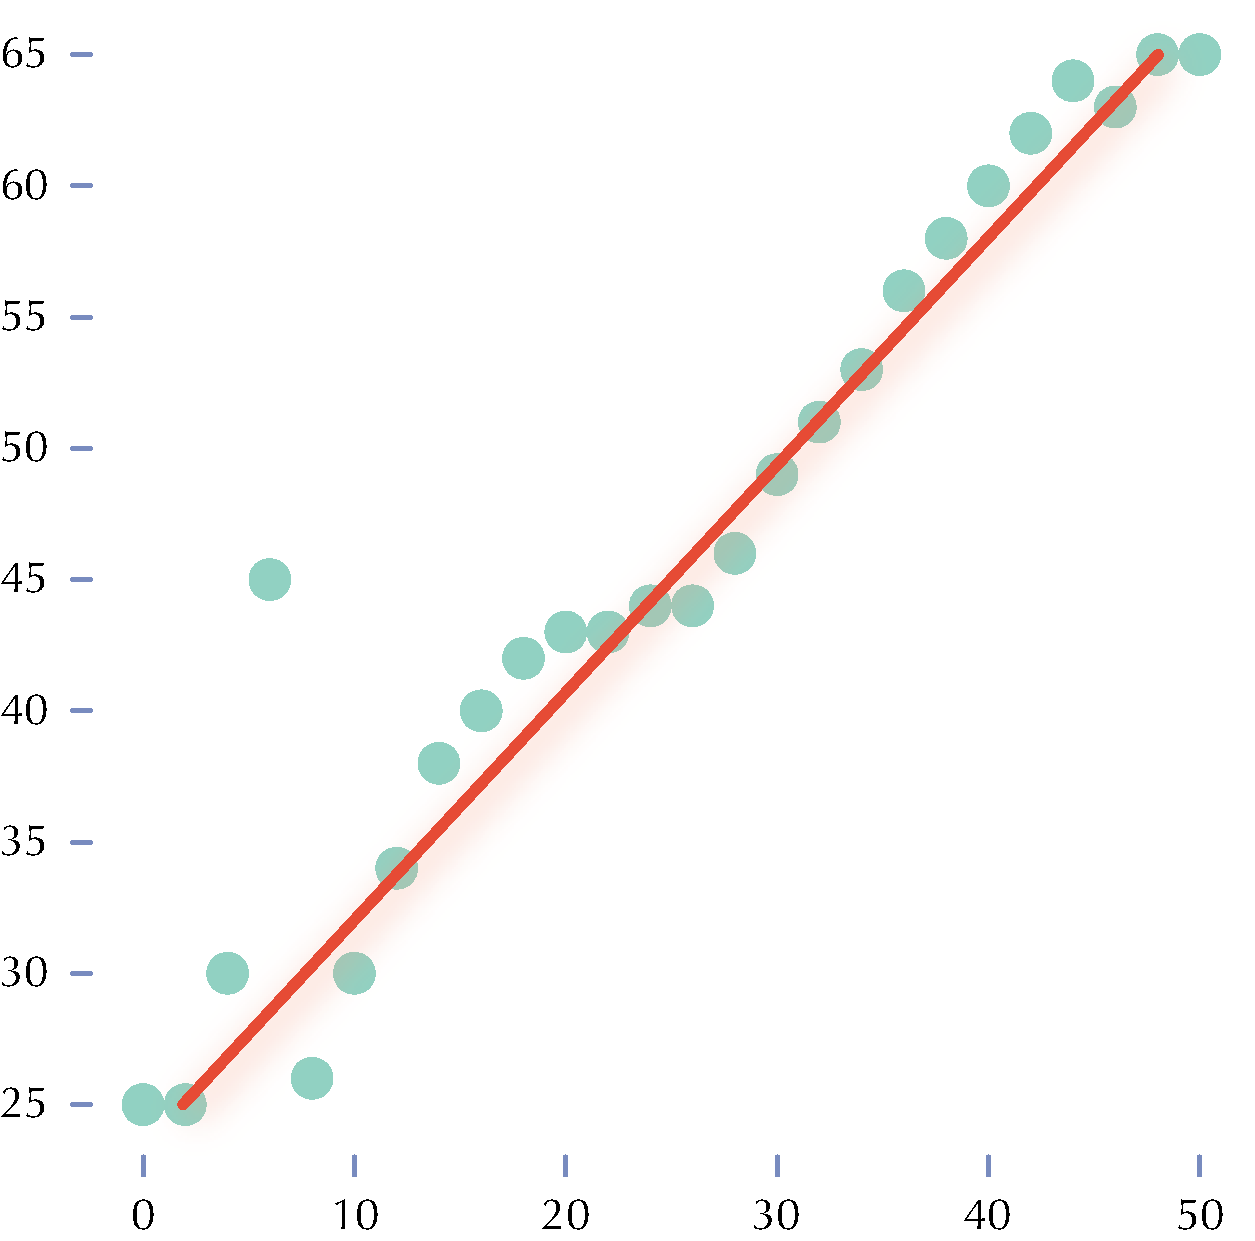
\includegraphics[width=\fcimagew]{src/assets/images/f-c-relationship.pdf}};
    \end{scope}
        
\end{tikzpicture}
    \caption{Caption}
    \label{fig:my_label}
\end{figure}

The Theil–Sen estimator defines the slope of the fitted line $\fcslope \in \mathbb{R}$ as the median of all possible slopes between pairs of points from the frequency-current graph:
\begin{equation}
    \fcslope = \median_{
        \tfrsimulation_i, \tfrsimulation_j \in \tfrsimulations \times \tfrsimulations
    } \left( 
        \frac{
            \domgammafreq_{\tfrsimulation_i} - \domgammafreq_{\tfrsimulation_j}
        }{
            I_{\ex, \tfrsimulation_i} - I_{\ex, \tfrsimulation_j}
        } 
    \right)
\end{equation}
To compute the intercept $\fcintercept \in \mathbb{R}$, the estimator uses the average values along the axes and the previously computed slope:
\begin{equation}
    \fcintercept = 
    \frac{1}{|\tfrsimulations|}
    \sum_{\tfrsimulation \in \tfrsimulations}
    \domgammafreq_\tfrsimulation
    -
    \frac{\fcslope}{|\tfrsimulations|}
    \sum_{\tfrsimulation \in \tfrsimulations}
    I_{\ex, \tfrsimulation}
\end{equation}

Knowing the slope of the linear relationship between the frequency and current, the current from external stimulus to the excitatory neurons in a PING network $\pingnet$ can be defined as follows:
\begin{equation}
    I_{\stim, \pingnet} = \fcslope \cdot f_\pingnet + \fcintercept.
\end{equation}
The derived values for $\fcslope$ and $\fcintercept$ are shown in Table ???.

\todo{include table ??? and figure ???}
\subsection{Cortical coordinates}
\label{sec:cortical-coords}

The receptive field is the region of the visual field to which a given neuron in the visual cortex responds. As shown in Figure \ref{fig:receptive-field}, it varies in size and shape depending on the distance from the fovea and occupies a three-dimensional space in the visual cortex. Therefore, when a two-dimensional stimulus is projected onto the receptive field, it becomes distorted, and a non-linear mapping is required to predict its location in the visual cortex.

To account for this distortion, the dipole map model is used \cite{Schwartz1980, Polimeni2006}. It is based on the idea that the visual field is represented by a set of dipoles, which are pairs of opposite poles on the surface of the visual field. The dipoles are mapped to the visual cortex using a complex-logarithm transformation, which accounts for the distortion caused by the varying size and shape of the receptive fields.

Let $\cmap: \mathbb{R}^2 \to \mathbb{R}^2$ be the function that maps the coordinates of a grid element (the PING network) from the visual field to the visual cortex. Let $\eccangle: V \to \left[ 0, \frac{\pi}{2} \right]$ be the angle between the horizontal axis and the line passing through points $\stimcenter$ and $(\patchstart + \centr(v))$. The function $\cmap$ is then defined using the complex-logarithm transformation as follows:
\begin{equation}
\begin{gathered}
    Z_v = \ecc_v \cdot \exp(\complexi \cdot \cortalpha \cdot \eccangle_v). 
    \\
    W_v = \cortk \cdot \log \left( 
        \frac{Z_v + \corta}{Z_v + \cortb}
    \right) - \cortk \cdot \log \left( 
        \frac{\corta}{\cortb}
    \right).
    \\
    \cmap(v) = (\Re(W_v), \Im(W_v)).
\end{gathered}
\end{equation}
The parameters $\cortk, \corta, \cortb$, and $\cortalpha$ are constants that determine the specific form of the transformation. 
The parameter $\cortk$ is a scaling factor that determines the overall size of the mapped dipoles, $\corta$ and $\cortb$ are constants that determine the dipoles' shape, and $\cortalpha$ is a rotation factor that determines the dipoles' orientation in V1.
The values of these parameters are determined through empirical studies (see Table \ref{tab:cortical-coords-params}).
An example of the transformation is visualized in Figure \ref{fig:coords-transformation}.

\begin{table}[!htp]
    \centering
    \begin{tabular}{|
>{\columncolor{table-color}}c |c|c|}
\hline
\textbf{Parameter} & {\cellcolor{table-color}\textbf{Value}}  \\ \hline
$\pmb{\cortk}$ & $15$ \\ \hline
$\pmb{\corta}$ & $0.7$ \\ \hline
$\pmb{\cortb}$ & $80$ \\ \hline
$\pmb{\cortalpha}$ & $0.9$ \\ \hline
\end{tabular}
    \caption[Coordinates conversion parameters]{Parameters for coordinates conversion \cite{Polimeni2005}.}
    \label{tab:cortical-coords-params}
\end{table}

\begin{figure}[!htp]
    \centering
    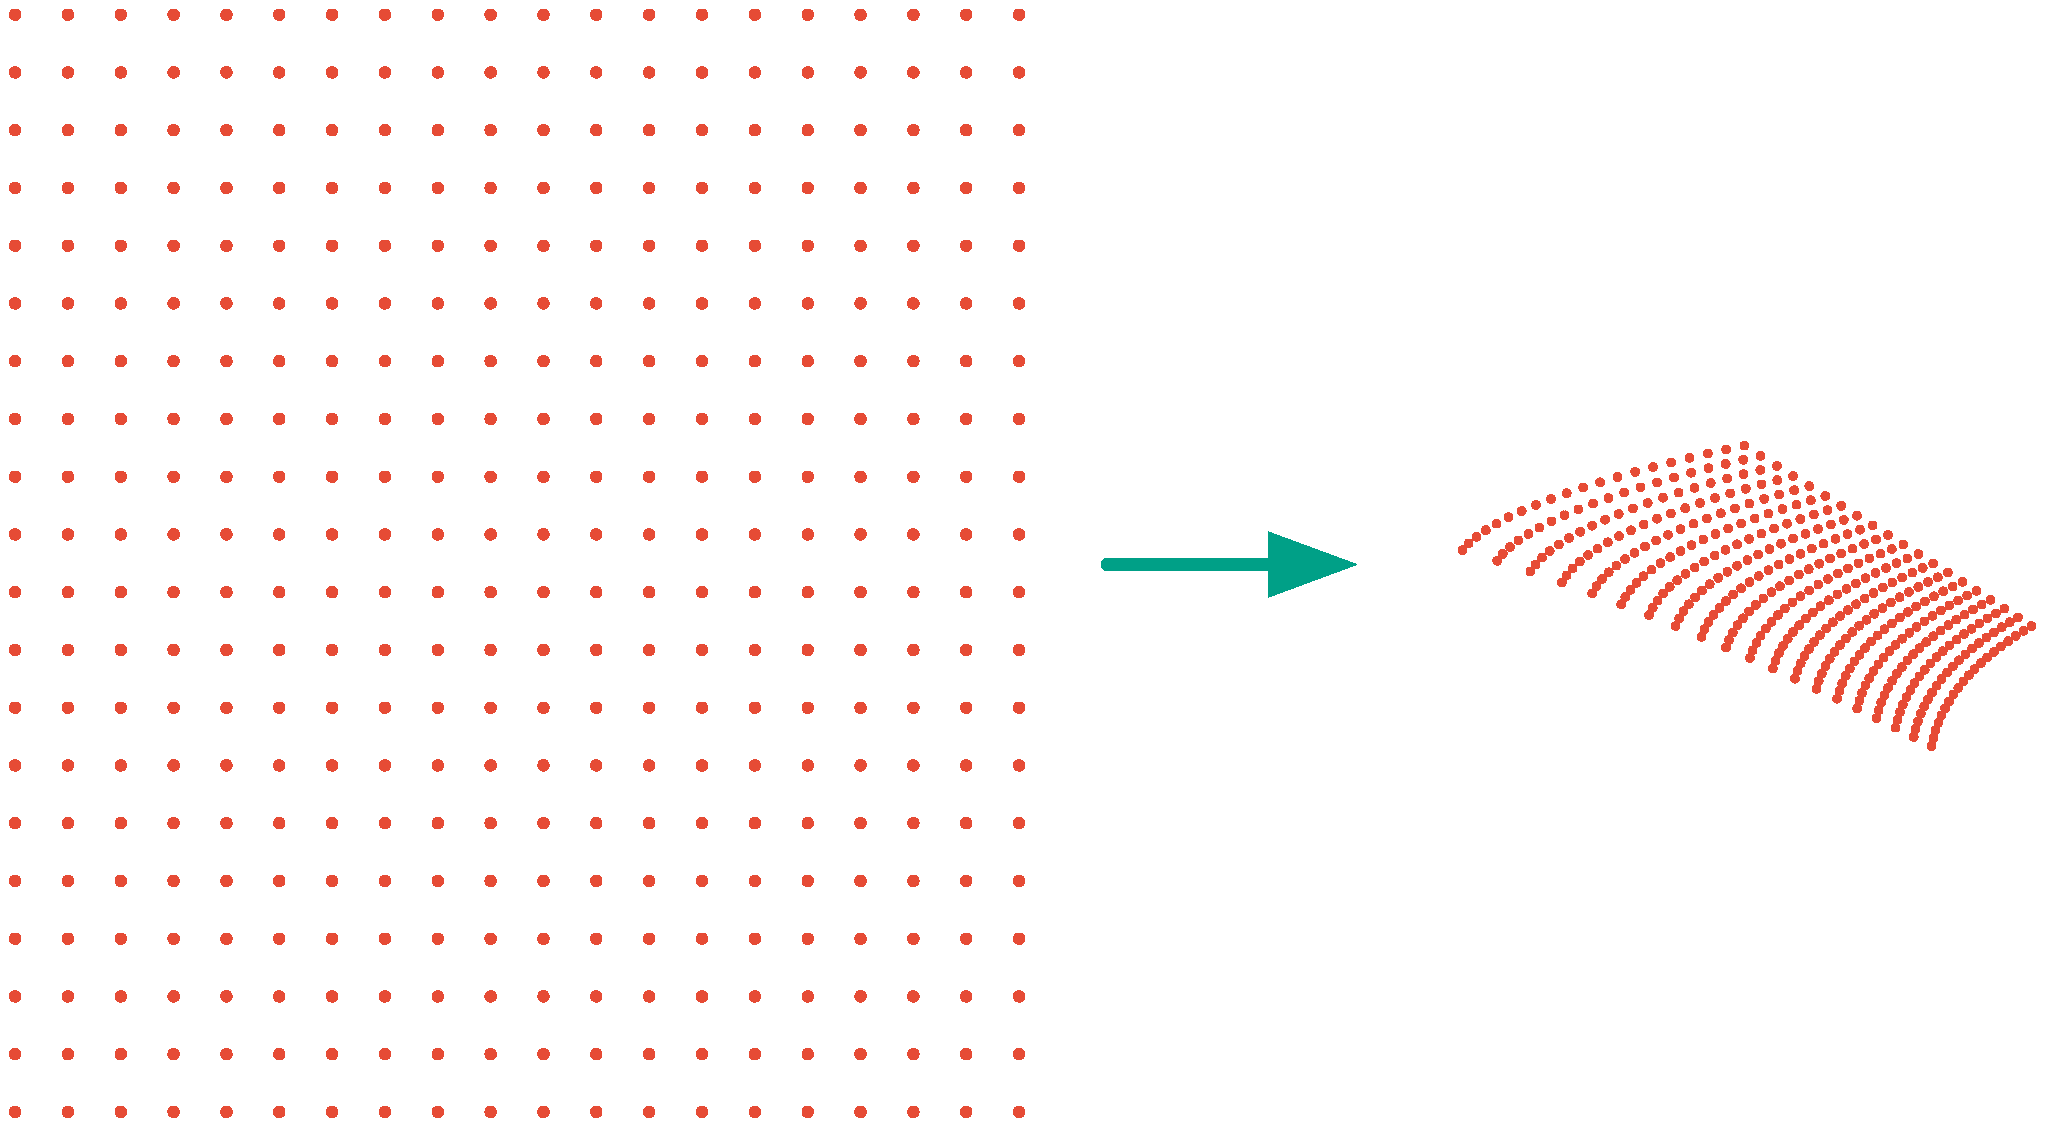
\includegraphics[width=0.7\textwidth]{src/assets/images/coords.pdf}
    \caption[Coordinates tranformation]{Transformation from visual to cortical coordinates for the 20 $\times$ 20 network.}
    \label{fig:coords-transformation}
\end{figure}
